%==============================
\subsection{Overall Analyses}\label{subsec:overall}
%==============================
\begin{figure*}[t!]
  \centering
  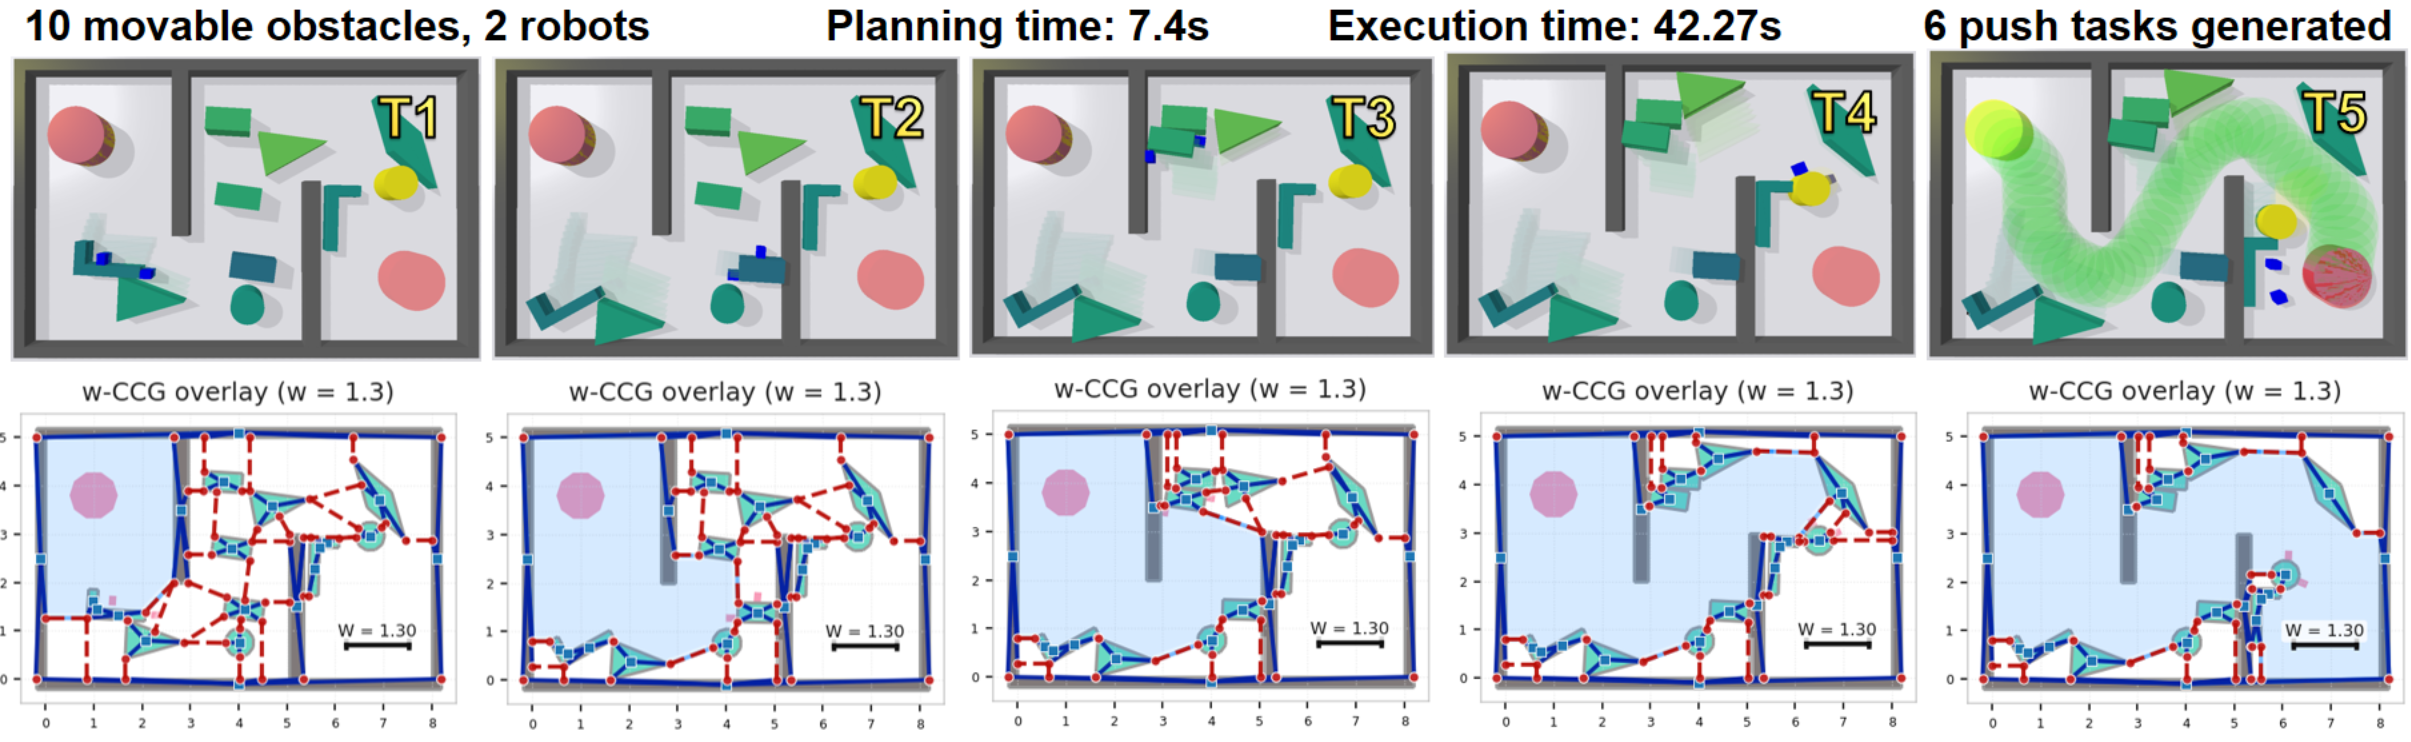
\includegraphics[width=0.95\linewidth]{figures/sim_exp.png}
  \vspace{-2mm}
\caption{Execution--planning alignment in the main scenario. 
\textbf{Top:} five PyBullet snapshots of the scene. 
\textbf{Bottom:} corresponding WCCG with the start face highlighted as a translucent blue polygon.
The task moves a cylindrical object from the start \(S=(1,4)\) to the goal \(G=(7,2)\). 
In the final snapshot, the start face contains \(G\), 
consistent with the green execution trajectory in the top row, 
confirming successful completion from \(S\) to \(G\). 
}
 \vspace{-4mm}
\end{figure*}


\subsubsection{Execution and Online Adaptation}\label{subsec:execute}
The output of the hybrid search is a pushing schedule
$\pi=\{\tau_1,\cdots,\tau_K\}$, where each $\tau_k$ specifies a target gap, a
short-horizon velocity $\mathbf{v}_k\triangleq(v_x,v_y,\omega)$, and a contact
mode $\boldsymbol{\xi}_k$. Execution proceeds sequentially under a hybrid
controller that alternates between transition and pushing phases.

During transition, robots plan collision-free paths in the
instantaneous freespace $\widehat{\mathcal{W}}(t)$ to reach their designated
contact points. If two paths are imminently head-on, the associated`
contacts are swapped to avoid deadlock.
During pushing, the commanded velocity $\mathbf{v}_k$ is integrated to form a
short reference trajectory for the manipulated obstacle. This trajectory is
mapped to per-robot contact states using $\boldsymbol{\xi}_k$, and each robot
$R_n$ executes proportional velocity control:
\[
\mathbf{v}_n = K_{\!p}\!\left(\widehat{\mathbf{p}}^{\,\text{c}}_n - \mathbf{p}^{\text{c}}_n\right),
\qquad
\omega_n = K_{\!r}\!\left(\widehat{\psi}^{\,\text{c}}_n - \psi^{\text{c}}_n\right),
\]
where $(\widehat{\mathbf{p}}^{\,\text{c}}_n,\widehat{\psi}^{\,\text{c}}_n)$ are
the reference contact states, $(\mathbf{p}^{\text{c}}_n,\psi^{\text{c}}_n)$ are
the measured states, and $K_{\!p},K_{\!r}>0$ are control gains. Small offsets
are adapted online to compensate for yaw drift and maintain stable contact.

Execution is monitored continuously. Transition feasibility is checked by
timeouts, while pushing is monitored by early-stop tests. If the commanded
widening succeeds, execution advances to $\tau_{k+1}$; otherwise, the
executor returns control to the planner with the current state. At a lower rate,
the WCCG is rebuilt and the execution terminates immediately once a
$W$--clear path $\mathcal{P}^W_\texttt{V}$ exists between
$\mathbf{s}_\texttt{V}^{\texttt{S}}$ and $\mathbf{s}_\texttt{V}^{\texttt{G}}$.

\begin{remark}[Endpoint Booster]
The $W$--CCG criterion of~\eqref{eq:wccg_criterion} may be conservative near
the endpoints. If connectivity holds but the disks
$\mathbb{B}_{W/2}(\mathbf{s}_\texttt{V}^{\texttt{S}})$ or
$\mathbb{B}_{W/2}(\mathbf{s}_\texttt{V}^{\texttt{G}})$ intersect obstacles, the
planner generates a small set of auxiliary pushes directed away from the
endpoints. These pushes clear the disks and allow execution to proceed.
\hfill$\blacksquare$
\end{remark}

%----------------------------------------------
\subsubsection{Computational Complexity}\label{subsubsec:complexity}
The cost of each node expansion is dominated by simulation of pushing
strategies. Construction of the $W$--clearance graph $\mathcal{G}_W$ and the
associated connectivity tests scale nearly linearly in the number of movable
obstacles $|\boldsymbol{\Omega}|$, while gap ranking by presearch
(Sec.~\ref{subsec:gap}) is lightweight because it is limited to a small subset
of frontier gaps. At expansion, only a fraction of the strategies in
$\mathsf{Rank}(\nu)$ survive the geometric quick-pass and early-stop checks,
which shortens the horizon of the simulator calls defined by
$\mathsf{EvalSim}$. Parallel execution of these simulations across multiple
workers reduces the effective cost nearly linearly until communication overhead
is reached. Deferred expansion further improves efficiency by distributing the
evaluation of $\mathsf{Rank}(\nu)$ across iterations, avoiding redundant
restarts and keeping the priority queue focused on promising frontiers.


%----------------------------------------------
\subsubsection{Generalization}\label{subsec:general}
The framework admits several natural extensions:
(I) \textit{Heterogeneous teams.} The controller structure admits per-robot gain
tuning, and mode priors can be augmented with robot-specific constraints.
This enables heterogeneous robots to cooperate within the same framework;
(II) \textit{Concurrent pushing.} While the executor applies one push task at a
time, the framework can be extended to allow concurrent pushing of multiple
obstacles. Such an extension requires multi-object mode generation and
transition planning to account for inter-robot conflicts;
(III) \textit{Dynamic environments.} Periodic $W$--connectivity checks and
on-demand re-planning enable adaptation to moderate disturbances such as object
drift or unmodeled contacts. The framework can therefore generalize to settings
where the environment changes gradually during execution.
